\begin{figure}
\begin{center}
    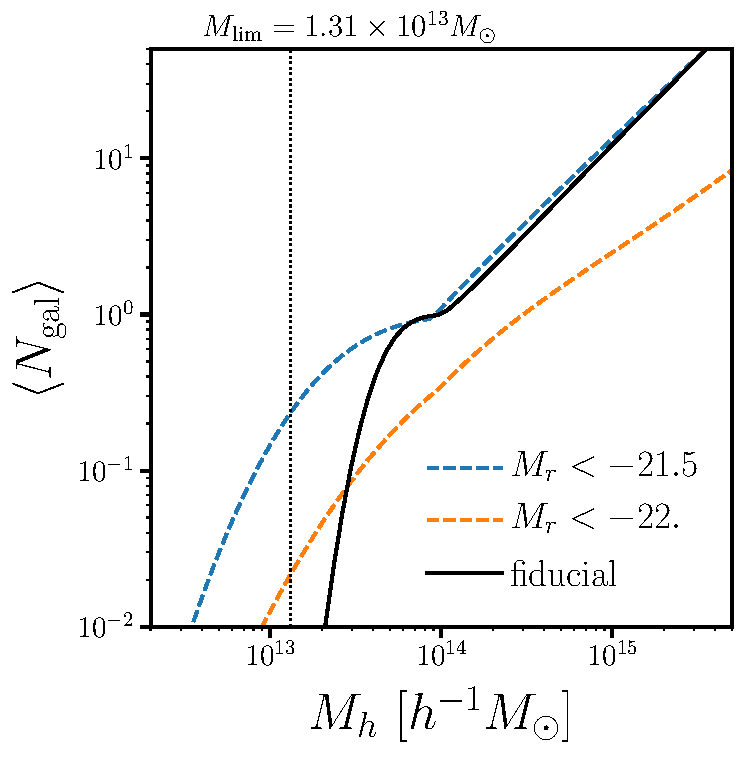
\includegraphics[width=0.45\textwidth]{figs/hod_fid.pdf} 
    \caption{The halo occupation our fiducial HOD model (black).
    }\label{fig:hod}
\end{center}
\end{figure}

\section{Halo Occupation Distribution} \label{sec:hod}  
We're interested in quantifying the information content of the galaxy bispectrum. 
With a perturbation theory approach, this would involve incorporating a bias model 
for galaxies~\citep[\emph{e.g.}][]{sefusatti2006, yankelevich2019, chudaykin2019}.
Perturbation theory approaches, however, break down on small scales and limit
the constraining power from nonlinear regime. Instead, in our simulation based 
approach we use the halo occupation distribution (HOD) framework~\citep[\emph{e.g.}][]{zheng2005,leauthaud2012,tinker2013,zentner2016,vakili2019}.% Berlind & Weinberg 2002; Peacock & Smith 2000; Seljak 2000; Benson et al. 2000; White et al. 2001; Cooray & Sheth 2002 
HOD models statistically populate galaxies in dark matter halos by specifying
the probability of a given halo hosting a certain number of galaxies. This 
statistical prescription for connecting galaxies to halos has been remarkably 
successful in reproducing the observational statistics of galaxies (\emph{e.g.} 
galaxy clustering) and, as a result, is the standard approach for constructing 
simulated galaxy mock catalogs in galaxy clustering analyses to estimate covariance 
matrices and test systematic effects~\citep[\emph{e.g.}][]{rodriguez-torres, mock challenge paper}. 
More importantly, HOD models in simulations for build galaxy clustering 
emulators~\citep[see the Aemulus project][]{zhai2018}. Emulation, as we mention above, 
is one of the most promising approaches for modeling small scale galaxy clustering 
and is what we're trying to forecast in this work. 

In the simplest HOD models, the probability of a given halo hosting $N$ galaxies 
of a certain class is dictated by its halo mass --- $P(N|M_h)$~\citep[\emph{e.g.}][]{zheng2007}. 
We use the standard $P(N|M_h)$ model from \cite{zheng2007}, which has been 
ubiquitously used in galaxy clustering analyses~\citep[\emph{e.g.}][]{citecite}. 
The model specifies the number of central and satellite galaxies in halos based 
on 
\beq
\langle N_{\rm cen} \rangle  = \frac{1}{2}\Bigg[1 + {\rm erf}\bigg(\frac{\log M_h - \log M_{\rm min}}{\sigma_{\log M}}\bigg) \Bigg]
\eeq
\beq
\langle N_{\rm sat} \rangle = \langle N_{\rm cen} \rangle \bigg(\frac{M_h - M_0}{M_1}^\alpha \bigg).
\eeq
\todo{
    describe $M_{\rm min}$, $\sigma_{\log M}$, $M_0$, $M_1$, $\alpha$. describe 
    how we actually assign the galaxy positions and velocities.  
}

In the \cite{zheng2007} model, the number of galaxies in a halo depend soley on $M_h$. 
However, if a secondary halo property is correlated with the spatial distribution of 
halos then there's assembly bias \todo{(citecite)}. 
If unaccounted for in the HOD model and not properly marginalized, this can possibly 
impact the cosmological parameter constraints. \cite{vakli2019}, however, find little 
evidence for assembly bias in the SDSS -21, -21.5 samples. Therefore, in this work
we use the standard \cite{zheng2007} model and assume it is sufficient for modeling 
galaxy bias. 

\bitem
\item description of the halo mass constraints we're dealing with and how this prevents 
    us from directly using best-fit HOD parameters from the literature. In fact, due
    to this constraint we modify the HOD parameters.
\item plots showing how our HOD choice compares to HODs of the SDSS samples. Some handwavy
    arguments about how it shouldn't matter too much. 
\eitem
